\documentclass{beamer}
\usepackage[english]{babel}
\usetheme{CambridgeUS}

\usepackage{caption}
\captionsetup{tableposition=top,figureposition=bottom,font=small}
\usepackage{graphicx}
\usepackage{subfig}
\usepackage{grffile}
\usepackage{booktabs}
\usepackage[absolute,overlay]{textpos}
\usepackage[noend,noline,tworuled]{algorithm2e}
\usepackage{minted}
\usepackage{calc}
\usepackage{xcolor}

\setlength{\parskip}{\smallskipamount}

\setbeamertemplate{navigation symbols}{}

\title[]{Screen Space Ambient Occlusion \\\small A WebGL-three.js implementation}

\newsavebox{\authbox}
\sbox{\authbox}{
    \centering
    \begin{minipage}{0.45\linewidth}
        \centering\normalsize
        Ivan Prosperi
    \end{minipage}
}

\author[Ivan Prosperi]{
    \texorpdfstring{\usebox{\authbox}}{Ivan Prosperi}}
\institute[]{Universit\`a degli Studi di Firenze}
\date{}
\logo{\textcolor{black}{\includegraphics[width=0.10\textwidth]{images/logo_unifi/stemma_grigio.pdf}}}

\AtBeginSection{%
    \begin{frame}
    \tableofcontents[currentsection,subsectionstyle=show/show/hide]
\end{frame}
}

%\let\nvec\vec
%\def\vec#1{\nvec{\vphantom t\smash{#1}}}
\newcommand{\textplus}{\raisebox{.1\height}{\scalebox{.9}{\texttt{+}}}}
\newcommand{\transform}[1]{$ \xrightarrow{\text{#1}} $}
\newcommand{\redtext}[1]{\textcolor{myred}{#1}}
\definecolor{myred}{RGB}{204, 0, 0}
\begin{document}
\definecolor{bg}{rgb}{0.95,0.95,0.95}
\newcommand{\glslvar}[1]{\mintinline[bgcolor=bg]{glsl}{#1}}

\begin{frame}
    \titlepage
    \centering
    Computer Graphics \& 3D Project Report
\end{frame}

\begin{frame}
    \frametitle{Table of contents}
    \tableofcontents[subsubsectionstyle=hide]
\end{frame}

% ##################### START #####################
\section{Introduction}

\subsection{Ambient Occlusion}

\begin{frame}
\frametitle{Ambient Occlusion}
% cosa è, immagini con/senza ao
Ambient occlusion is a shading technique that computes the \emph{degree of exposure} to ambient light in a 3D scene:
\begin{itemize}
    \item \redtext{open surfaces}, planar geometries, ``floating'' geometries: fully exposed to ambient light
    \item \redtext{hidden geometries}, corners, tight gaps between objects, creases: appear shaded in real life, ambient light does not reach them at full intensity
\end{itemize}

\end{frame}

\begin{frame}
\frametitle{Ambient Occlusion Effects}
\begin{figure}
    \centering
    \includegraphics[width=0.8\linewidth]{images/B-25_raw.png}
    \caption{3D object with raw material.\footnotemark}
\end{figure}

\vspace*{-8px}
\footnotetext{Landis, H. Production-Ready Global Illumination (2004).}
\end{frame}

\begin{frame}
\frametitle{Ambient Occlusion Effects}
\begin{figure}
    \centering
    \includegraphics[width=0.8\linewidth]{images/B-25_ao.png}
    \caption{The same object with ambient occlusion applied.}
\end{figure}

\end{frame}

\subsection{Global Illumination}
\begin{frame}[allowframebreaks]
\frametitle{Global Illumination}
% cosa è, immagini indirect light + AO vera + citazione paper AO
% Dire che ao vera è fatta con indirect lighting di GI ma troppo
% costoso in caso di real time
\textbf{Global Illumination (GI)}:
\begin{itemize}
    \item \redtext{considers} physically correct light phenomena
    \item \redtext{is} a \underline{global method}: illumination at each point is a function of other geometry in the scene
    \item \redtext{accounts} for light rays (possibly infinite) bounces
    \item \redtext{implements} indirect illumination
    \item \redtext{comprises} reflection, refraction, shadows, diffuse inter-reflections, caustics, etc
\end{itemize}

Ambient occlusion approximates some aspects of Global Illumination.

%\end{frame}
\framebreak
%\begin{frame}
%\frametitle{Global Illumination II}
\begin{figure}
    \centering
    \includegraphics[width=0.9\linewidth]{images/gi_room.jpg}
\end{figure}
%\end{frame}
\framebreak
%\begin{frame}
%\frametitle{Global Illumination III}
Global illumination limits:
\begin{itemize}
    \item a pixel color value depends on the entire scene
    \item light calculation involves solving complex equations
    \item no algorithm exists to implement GI as a whole
\end{itemize}

Furthermore, current real-time graphics hardware is mostly based on rasterization $ \Rightarrow $ ideal for direct illumination computation.

Therefore, \textbf{GI is not reproducible in real time rendering} with the current technologies and hardware.
\end{frame}

\begin{frame}%[allowframebreaks]
\frametitle{Multipass Rendering}
% Far vedere esempio di multipass rendering
% Scrivere tipo "used for shadow mapping, normal mapping, etc"
Multipass rendering (and deferred shading) are employed as low-cost approximations for GI effects:
\begin{itemize}
    \item shadow mapping
    \item soft shadows
    \item reflection mapping
    \item light mapping
    \item \textbf{ambient occlusion}
\end{itemize}

%\begin{figure}
%    \centering
%    \includegraphics[width=0.9\linewidth]{images/reflection_map.jpg}
%\end{figure}

\end{frame}


\section{Screen Space Ambient Occlusion}

\subsection{Principles}

\begin{frame}
\frametitle{Screen Space Ambient Occlusion}
% crytek-crysis 2007
Screen Space Ambient Occlusion (SSAO):
\begin{itemize}
    \item first approach to real time AO
    \item developed at \emph{Crytek GmbH} and included in \emph{CryEngine 2}
    \item used in \emph{Crysis} (2007)
\end{itemize}

\begin{columns}
    \begin{column}{0.4\linewidth}
        \begin{figure}
        \centering
        \subfloat{
\includegraphics[width=0.5\linewidth]{images/crytek_logo.pdf}} \\
        \subfloat{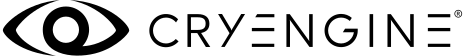
\includegraphics[width=0.8\linewidth]{images/cryengine_logo.pdf}}
        \end{figure}
    \end{column}

    \begin{column}{0.4\linewidth}
        \begin{figure}
        \centering
        \includegraphics[width=\linewidth]{images/crysis_cover.png}
        \end{figure}
    \end{column}
\end{columns}

\end{frame}

\begin{frame}
\frametitle{SSAO in Crysis I}
% mettere immagine crysis coreano + tank + muro dietro
\begin{figure}
    \centering
    \includegraphics[width=0.8\linewidth]{images/ssao_crysis_gameplay.png}
\end{figure}
\end{frame}

\begin{frame}
\frametitle{SSAO in Crysis II}
\begin{figure}
    \centering
    \includegraphics[width=0.8\linewidth]{images/ssao_tank.jpg}
\end{figure}

\end{frame}

\begin{frame}
\frametitle{Screen Space}
SSAO is a \emph{screen space} (ss) technique:
\begin{itemize}
    \item uses \redtext{deferred rendering} to split geometry render from light computation:
    \begin{itemize}
        \item pass 1: \redtext{render geometry/depth} in off-screen buffers (g-buffer)
        \item pass 2: \redtext{use g-buffers} as textures to apply lighting
    \end{itemize}
    \item ss effects applied in pass 2 $ \Rightarrow $ screen space resolution dependent
    \item application of ss techniques does not depend on scene complexity (roughly)
\end{itemize}
\end{frame}

%\begin{frame}
%\frametitle{Deferred Rendering Pipeline}
%\begin{figure}
%    \centering
%    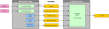
\includegraphics[width=0.9\linewidth]{images/deferred_rendering.pdf}
%\end{figure}
%
%\SetKwFor{ForEach}{for each}{}{}
%\begin{columns}
%    \begin{column}[t]{0.44\linewidth}
%        Forward rendering: $\mathcal{O}(N L R)$
%        \smaller
%        \begin{algorithm}[H]
%            \ForEach{object}{
%                \ForEach{fragment}{
%                    \ForEach{light}{
%                        compute lighting\;
%                    }
%                }
%            }
%        \end{algorithm}
%    \end{column}
%    
%    \begin{column}[t]{0.44\linewidth}
%        Deferred rendering: $\mathcal{O}((N{+}L)R)$
%        \smaller
%        \begin{algorithm}[H]
%            \ForEach{object}{
%                \ForEach{fragment}{
%                    fill g-buffer\;
%                }
%            }
%            \ForEach{light}{
%                \ForEach{fragment}{
%                    fetch g-buffer\;
%                    compute lighting\;
%                }
%            }
%        \end{algorithm}
%    \end{column}
%\end{columns}
%\end{frame}

\begin{frame}
\frametitle{SSAO Approach}
SSAO fundamental ideas:
\begin{itemize}
    \item leverage deferred rendering (\redtext{post processing})
    \item use available geometry info to \redtext{approximate indirect lighting}
    \item computation of a \redtext{screen space occlusion map} based on geometries surrounding current rasterized fragment
    \item \redtext{blending} of occlusion map with ambient lighting to shade appropriate portions of the image
    \item (use of depth buffer for geometry reconstruction\textemdash{}more on this later)
\end{itemize}
\end{frame}

\begin{frame}
\frametitle{Crytek SSAO}
Crytek's original implementation was never released. High level description available in  \emph{``Finding Next Gen\textemdash{}CryEngine 2''} paper from Crytek.

%Algorithm's high level pseudocode:
%\RestyleAlgo{plain}
\SetKwFor{ForEach}{for each}{}{}
%\SetKwIF\If{cond}{Then’s text}
\SetKwIF{If}{ElseIf}{Else}{if}{}{else if}{else}{endif}
\begin{algorithm}[H]
    render geometry\;
    \ForEach{fragment \textup{in geometry g-buffer}}{
        sample \emph{fragment}'s view space position\;
        sample some points in view space neighborhood\;
        \ForEach{sample}{
            project \emph{sample} in clip space\;
            \If{sample \textup{is behind rasterized geometry}}{
                increment occlusion for current \emph{fragment}\;
            }
        }
        average occlusion for current \emph{fragment} on all \emph{samples}\;
        write $ (1 - \mathit{occlusion}) $ to texture\;
    }
    blend AO map with ambient lighting\;
    \caption{SSAO high level pseudocode.}
\end{algorithm}

\end{frame}

\begin{frame}
\frametitle{SSAO Scheme}
\begin{figure}
    \centering
    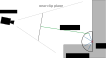
\includegraphics[width=0.9\linewidth]{images/ssao_scheme}
\end{figure}

\end{frame}

\subsection{View Space Reconstruction}
\begin{frame}
\frametitle{Reconstruction From Depth}
Base SSAO:
\begin{itemize}
    \item \redtext{pass} a view-space position texture to SSAO shader
    \item \redtext{heavy on memory} and bandwidth, \redtext{no processing}
\end{itemize}

Extension:
\begin{itemize}
    \item \redtext{reconstruct} view-space position from depth
    \item \redtext{no memory footprint} (use depth buffer), \redtext{requires processing} in shaders
\end{itemize}
\end{frame}

%\begin{frame}
%
%\frametitle{Background: OpenGL pipeline}
%Coordinates: object \transform{MVP} clip \transform{clip/w-divide} NDC \transform{viewport} window.
%\begin{figure}
%    \centering
%    \includegraphics[width=0.9\linewidth]{images/coordinate_systems.png}
%\end{figure}
%
%\end{frame}

\begin{frame}
\frametitle{View Space Z from Depth Buffer}
\label{frame:viewspace-from-depth-buffer}

Transformation of z (\redtext{view space $ \mapsto $ NDC}):
\[
z_{ndc} = \dfrac{z_{clip}}{w_{clip}} = \dfrac{-\dfrac{f+n}{f-n} z_e -2 \dfrac{fn}{f-n}}{-z_e} = \dfrac{\beta z_e + \gamma}{-z_e}
\]

Depth value written in depth buffer (\redtext{NDC $ \mapsto $ depth}):
\[
d = z_{ndc} * 0.5 + 0.5 = \dfrac{(\beta - 1) z_e + \gamma}{-2z_e}
\]

View space reconstruction from depth buffer (\redtext{depth $ \mapsto $ view space}):

\[
z_e = \dfrac{\gamma}{1-2d-\beta}
\]
\end{frame}


\begin{frame}
\frametitle{View Space X and Y}
Transformation of x (\redtext{view space $ \mapsto $ NDC}):
\[
x_{ndc} = \dfrac{x_{clip}}{w_{clip}} = \dfrac{x_e}{-z_e \alpha \tan(fov/2)}, \quad -1 \le x_{ndc} \le 1
\]

\newlength{\halfdiff}
\setlength\halfdiff{( \widthof{$ \dfrac{x_e}{-z_e \alpha \tan(fov/2)} $} - \widthof{$x_e$} ) / 2}
It holds:
\begin{alignat*}{2}
-1 &\le \dfrac{x_e}{-z_e \alpha \tan(fov/2)} &&\le 1 \\
-\alpha \tan(fov/2)\,z_e &\le \hspace{\halfdiff} x_e &&\le \alpha \tan(fov/2)\,z_e
\end{alignat*}

Extremal values: \redtext{corners} of the post-processing \redtext{full-screen quad}.

\end{frame}

\begin{frame}
\frametitle{View Ray}
\redtext{Solution}: 
\begin{itemize}
    \item construct a 2-dimensional vector, called \redtext{view ray}:
    \[
    \text{\redtext{view ray}} = \bigl(\alpha \tan(fov/2)\:x_{clip}, \tan(fov/2)\:y_{clip}\bigr)
    \]
    \item Let the hardware interpolate the view ray, then reconstruct position:
    \[
    \text{\redtext{view position}} = z_e \bigl(-\text{\redtext{view ray}}, 1\bigr)
                         = \bigl( x_e, y_e, z_e \bigr)
    \]
\end{itemize}

\end{frame}

\begin{frame}[fragile]
\frametitle{Vertex Shader}
\begin{minted}[bgcolor=bg,fontsize=\footnotesize]{glsl}
...
void main() {
    vec4 clip = MVP * vec4(position, 1.0);
    view_ray = vec3(-tan(hfov) * a * clip.x, -tan(hfov) * clip.y, 1.0);
    gl_Position = clip;
}

\end{minted}
where \glslvar{MVP} is the model-view-projection matrix, \glslvar{a} is the aspect ratio $ \alpha $ and \glslvar{hfov} is $ fov/2 $.


\end{frame}

\begin{frame}[fragile]
\frametitle{Fragment Shader}
\begin{minted}[bgcolor=bg,fontsize=\footnotesize]{glsl}
...
void main() {
    ...
    float depth = texture2D(depth_texture, tex_coords).x;
    float view_z = unproject_depth(depth);
    vec3 origin = view_ray * view_z;
    ...
\end{minted}
where \glslvar{origin} is the view space position of the geometry rasterized in the current fragment.

The function \glslvar{unproject_depth} applies the transformation (\redtext{depth~$ \mapsto $~view space}) defined on slide~\redtext{\ref{frame:viewspace-from-depth-buffer}}.

\end{frame}

\subsection{Implementation Details}

\begin{frame}[fragile]
\frametitle{Sample kernel}
\redtext{Uniform variable} in fragment shader:
\begin{minted}[bgcolor=bg,fontsize=\footnotesize]{glsl}
uniform vec3 sample_kernel[KERNEL_SIZE];
\end{minted}

For each vector, components are random numbers s.t.:
\begin{align*}
-1 & \le x \le 1 \\
-1 & \le y \le 1 \\
0 & \le z \le 1
\end{align*}

Forms a \redtext{hemisphere} centered in $ (0, 0, 0) $ (\redtext{tangent space}).

Must be \redtext{reoriented} inside the shader.
\end{frame}

\begin{frame}[fragile]
\frametitle{Non-Uniformly Distributed Samples}
Samples near the origin are more interesting.

\redtext{Accelerating interpolation function} to scale the samples:
\begin{minted}[bgcolor=bg,fontsize=\footnotesize]{c++}
float scale = (float)i / KERNEL_SIZE; // i is the loop variable
scale = lerp(0.1f, 1.0f, scale * scale);
sample *= scale;
\end{minted}

\vspace{0.3cm}

\begin{columns}
    \begin{column}{0.45\linewidth}
        \centering
        Uniform samples:
        \begin{figure}
            \centering
            \vspace{-1.8ex}%
            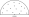
\includegraphics[width=0.7\linewidth]{images/sample_kernel_uniform.pdf}
        \end{figure}
    \end{column}
    
    \begin{column}{0.45\linewidth}
        \centering
        \redtext{Non uniform samples}:
        \begin{figure}
            \centering
            \vspace{-1.8ex}%
            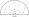
\includegraphics[width=0.7\linewidth]{images/sample_kernel_accel.pdf}
        \end{figure}
        
    \end{column}
\end{columns}

\end{frame}

\begin{frame}[fragile]
\frametitle{Random Kernel Rotations}
For convincing results: \redtext{high sampling rate} $ \Rightarrow $ Performance degradation.

\redtext{Solution}: use a random $ 4\times4 $ noise texture to \redtext{rotate} samples:
\begin{minted}[bgcolor=bg, fontsize=\footnotesize]{c++}
noise_texture[i] = Vector3(random(-1,1), random(-1,1), 0);
\end{minted}

\redtext{Tile} the texture over the entire screen:
\begin{minted}[bgcolor=bg, fontsize=\footnotesize]{c++}
glTexParameteri(GL_TEXTURE_2D, GL_TEXTURE_WRAP_S, GL_REPEAT);
glTexParameteri(GL_TEXTURE_2D, GL_TEXTURE_WRAP_T, GL_REPEAT);
\end{minted} 

\end{frame}

\begin{frame}
\frametitle{Samples Reorientation I}
Transform samples (\redtext{tangent space $ \mapsto $ view space}):
\begin{enumerate}
    \item compute an orthonormal base (normal, tangent, bitangent) from normal and noise vectors\footnotemark:
    \begin{gather*}
        \vec{\tau} = \vec{r} - (\vec{r} \cdot \vec{n}) \vec{n}, \quad \vec{t} = \dfrac{\vec{\tau}}{|\vec{\tau}|} \\
        \vec{b} = \vec{n} \times \vec{t}
    \end{gather*}
    \item Transform:
    \[
    \vec{v}_{\text{view-space}} = \text{TBN} \; \vec{v}_{\text{tangent-space}}, \quad
    \text{TBN} =
    \begin{bmatrix}
    \vec{t} & \vec{b} & \vec{n}
    \end{bmatrix} \in \mathbb{R}^{3\times3}
    \]
\end{enumerate}

%\vspace*{-8px}
\footnotetext{Gram–Schmidt process for orthonormalization.}
\end{frame}

\begin{frame}[fragile]
\frametitle{Sample Reorientation II}

TBN creation in fragment shader:
\begin{minted}[bgcolor=bg, fontsize=\footnotesize]{glsl}
vec3 tangent = normalize(noise - normal * dot(noise, normal));
vec3 bitangent = cross(normal, tangent);
mat3 tbn = mat3(tangent, bitangent, normal);
\end{minted}

\vspace{-0.2cm}
\begin{figure}
    \centering
    
\includegraphics[width=0.7\linewidth]{images/kernel_reorientation.pdf}
\end{figure}

\end{frame}

\begin{frame}[fragile]
\frametitle{Sample Reorientation III}
To get a sample's view position:
\begin{itemize}
    \item \redtext{reorient} sample
    \item \redtext{scale} sample to radius
    \item \redtext{translate} sample: add origin (fragment's view space position)
\end{itemize}
\begin{minted}[bgcolor=bg, fontsize=\footnotesize]{glsl}
float occlusion = 0.0;
for (int i = 0; i < KERNEL_SIZE; ++i) { // SSAO shader main loop
    vec3 sample_point = tbn * sample_kernel[i];
    sample_point = (sample_point * kernel_radius) + origin;
    ...
\end{minted}

\end{frame}

\begin{frame}[fragile]
\frametitle{Projection}
Steps:
\begin{itemize}
    \item \redtext{project} sample in clip space
    \item perform \redtext{perspective divide}
    \item \redtext{bias}, to get coordinates in $\ [0,1] $
\end{itemize}

\begin{minted}[bgcolor=bg, fontsize=\footnotesize]{glsl}
    vec4 sample_point_ndc = projection_matrix * vec4(sample_point, 1.0);
    sample_point_ndc.xy /= sample_point_ndc.w;
    vec2 sample_point_uv = sample_point_ndc.xy * 0.5 + 0.5;
    ...
\end{minted}

The variable \glslvar{sample_point_uv} represents the \redtext{texture coordinates} of the projected sample.

\end{frame}

\begin{frame}[fragile]
\frametitle{Depth Comparison}
\redtext{Compare}:
\begin{itemize}
    \item \redtext{depth buffer}'s depth value (true rasterized geometry)
    \item \redtext{sample}'s depth value
\end{itemize}

\begin{minted}[bgcolor=bg, fontsize=\footnotesize]{glsl}
    float real_depth = texture2D(t_depth, sample_point_uv).r;
    float linear_real_depth = unproject_depth(real_depth);
    float sample_depth = sample_point.z;
    
    float delta = linear_real_depth - sample_depth;
    ...
\end{minted}

Discriminate on \glslvar{delta} value whether this sample contributes to occlusion or not.
\end{frame}

\begin{frame}[fragile]
\frametitle{Occlusion Computation: Naive Approach}
Naive approach:
\begin{minted}[bgcolor=bg, fontsize=\footnotesize]{glsl}
    if (delta >= 0.0) {
        occlusion += 1.0;
    }
    ...
\end{minted}

\begin{columns}
    \begin{column}{0.45\linewidth}
        \redtext{Binary} valued occlusion:
        \begin{itemize}
            \item \redtext{too coarse}, might generate artifacts
            \item \redtext{overshadows} overlapping geometries, even if distant
        \end{itemize}
    \end{column}
    \begin{column}{0.45\linewidth}
        \begin{figure}
            \centering
            \includegraphics[width=0.8\linewidth]{images/occlusion_naive}
        \end{figure}
    \end{column}
\end{columns}

\end{frame}

\begin{frame}[fragile]
\frametitle{Occlusion Computation: Range Check}
Range check inclusion:
\begin{minted}[bgcolor=bg, fontsize=\footnotesize]{glsl}
    float range_check = abs(linear_real_depth - origin.z)
        < kernel_radius ? 1.0 : 0.0;
    occlusion += (delta >= 0.0 ? 1.0 : 0.0) * range_check;
    ...
\end{minted}

\begin{columns}
    \begin{column}{0.45\linewidth}
        \redtext{Binary} valued occlusion with range check:
        \begin{itemize}
            \item \redtext{still coarse}. Visible artifacts (see next slides)
            \item \redtext{solves} overshadowing of distant geometries 
        \end{itemize}
    \end{column}
    \begin{column}{0.45\linewidth}
        \begin{figure}
            \centering
            \includegraphics[width=0.8\linewidth]{images/occlusion_hard_range_check.png}
        \end{figure}
    \end{column}
\end{columns}

\end{frame}

\begin{frame}[fragile]
\frametitle{Occlusion Computation: Range Check (soft)}
Soft range check inclusion:
\begin{minted}[bgcolor=bg, fontsize=\footnotesize]{glsl}
    float value = kernel_radius / abs(linear_real_depth - origin.z);
    float range_check = smoothstep(0.0, 1.0, value);
    occlusion += (delta >= 0.0 ? 1.0 : 0.0) * range_check;
    ...
\end{minted}

\begin{columns}
    \begin{column}{0.45\linewidth}
        \redtext{Continuous} valued occlusion with range check:
        \begin{itemize}
            \item \redtext{finer} control: artifacts removed/attenuated
            \item \redtext{solves} overshadowing of distant geometries 
        \end{itemize}
    \end{column}
    \begin{column}{0.45\linewidth}
        \begin{figure}
            \centering
            \includegraphics[width=0.8\linewidth]{images/occlusion_soft_range_check.png}
        \end{figure}
    \end{column}
\end{columns}

\end{frame}

\begin{frame}[fragile]
\frametitle{Occlusion Computation: Range Check (soft) II}
Soft range check inclusion: removes artifacts.
\begin{minted}[bgcolor=bg, fontsize=\footnotesize]{glsl}
    float value = kernel_radius / abs(linear_real_depth - origin.z);
    float range_check = smoothstep(0.0, 1.0, value);
    occlusion += (delta >= 0.0 ? 1.0 : 0.0) * range_check;
    ...
\end{minted}

\begin{columns}
    \begin{column}{0.45\linewidth}
    \centering
        Hard range check:
        \begin{figure}
            \centering
            \vspace{-1ex}%
            \includegraphics[width=0.8\linewidth]{images/feet_hard_range_check.png}
        \end{figure}
    \end{column}

    \begin{column}{0.45\linewidth}
        \centering
        Soft range check
        \begin{figure}
            \centering
            \vspace{-1ex}%
            \includegraphics[width=0.8\linewidth]{images/feet_soft_range_check.png}
        \end{figure}
    \end{column}
\end{columns}

\end{frame}

\begin{frame}[fragile]
\frametitle{Distance Constraints}
Add constraints to avoid some artifacts:
\begin{itemize}
    \item constraints applied on \glslvar{delta} (geometry depth - sample depth)
    \item ability to tune the effect according to the scene
\end{itemize}

\begin{minted}[bgcolor=bg, fontsize=\footnotesize]{glsl}
    float value = kernel_radius / abs(linear_real_depth - origin.z);
    float range_check = smoothstep(0.0, 1.0, value);
    float constraints = (delta >= min_distance && delta < max_distance);
    occlusion += (constraints ? 1.0 : 0.0) * range_check;
    ...
\end{minted}
\end{frame}

\begin{frame}
\frametitle{Blur}
A blur pass is necessary to \redtext{filter} high frequency pattern introduced by noise texture.

Implemented in a second shader, applied after SSAO shader.

\vspace{0.6cm}

\begin{columns}
    \begin{column}{0.45\linewidth}
        \centering
        SSAO
        \begin{figure}
            \vspace{-1ex}%
            \includegraphics[width=0.7\linewidth]{images/no_blur.png}
        \end{figure}
    \end{column}
    
    \begin{column}{0.45\linewidth}
        \centering
        SSAO + Blur
        \begin{figure}
            \vspace{-1ex}%
            \includegraphics[width=0.7\linewidth]{images/blur.png}
        \end{figure}
    \end{column}
\end{columns}

\end{frame}


\section{Results}

\begin{frame}
\frametitle{Application}
A \redtext{web application} was created to show the results of the project.

Scene created with publicly available 3D models.
\vspace{0.6cm}
\begin{columns}
    \begin{column}[t]{0.45\linewidth}
        \redtext{Four views} available:
        \begin{itemize}
            \item complete
            \item beauty
            \item SSAO
            \item SSAO + blur
        \end{itemize}
    \end{column}

    \begin{column}[t]{0.45\linewidth}
        \redtext{Configurable parameters}:
        \begin{itemize}
            \item kernel radius
            \item minimum / maximum distances
            \item range check factor
            \item power factor
        \end{itemize}
    \end{column}

\end{columns}

\end{frame}

\newcommand{\resultwidth}{0.9\linewidth}

\begin{frame}
\frametitle{App: SSAO Layer}
\begin{figure}
    \centering
    \includegraphics[width=\resultwidth]{images/app_ssao}
\end{figure}

\end{frame}

\begin{frame}
\frametitle{App: Blur Layer}
\begin{figure}
    \centering
    \includegraphics[width=\resultwidth]{images/app_blur}
\end{figure}

\end{frame}

\begin{frame}
\frametitle{App: Beauty Layer}
\begin{figure}
    \centering
    \includegraphics[width=\resultwidth]{images/app_beauty}
\end{figure}

\end{frame}

\begin{frame}
\frametitle{App: Complete Layer}
\begin{figure}
    \centering
    \includegraphics[width=\resultwidth]{images/app_complete}
\end{figure}

\end{frame}

\section{Tools and Software}
\begin{frame}
\frametitle{Tools and Software}
% threejs webgl buildpack node/npm heroku eslint
The project was realized in \redtext{Javascript}, using the 3D graphics library \redtext{three.js} (\redtext{WebGL}).

\redtext{Node.js} and its package manager \redtext{npm} were used to provide dependency management and deployment.

The \redtext{Webpack} bundler was used to assemble the project.

Application hosted on \redtext{Heroku}.
\begin{figure}
    \centering
    
\includegraphics[width=0.6\linewidth]{images/software_logos.pdf}
\end{figure}


\end{frame}

\section{Conclusions}

\begin{frame}
\frametitle{Known Problems}
The encountered problems are those typical of SSAO technique:
\begin{itemize}
    \item halo effect on object borders (\redtext{bleeding}): due to ``blind'' blur
    \item high number of \redtext{parameters}, hard to find a global optimum
    \item SSAO effects greatly depends on scene scale and complexity
\end{itemize}

Possible solution for SSAO bleeding: \redtext{depth-aware blur}.

More recently, some advanced algorithms have been developed, which overcome SSAO criticalities: HBAO/HBAO\textplus, SSDO, RTAO, etc.
\end{frame}



\begin{frame}
\frametitle{Conclusions}
Features of this project:
\begin{itemize}
    \item \redtext{fully functioning} project realized with latest technologies
    \item \redtext{deployed} on a public hosting service
    \item showcases the Screen Space Ambient Occlusion technique
    \item includes \redtext{fixes and improvements} over the original method
    \item adopts a \redtext{depth reconstruction} methodology
\end{itemize}

Links to the project repository and online version:
\begin{itemize}
    \item \redtext{\underline{\url{https://github.com/ivan94fi/cg3d_project_ssao}}}
    \item \redtext{\underline{\url{https://cg3d-project-ssao.herokuapp.com/}}}
\end{itemize}

\end{frame}

% ##################### END #####################

\end{document}